\section{Real-time Garbage Collection}


This section is based on a paper published at JTRES 2007
\cite{jop:scjgc}.

\emph{TODO: edit some sections and add a different related work
part. Add GC scheduling and other GC related stuff.}

The Real-time Specification for Java and the upcoming, and more
restricted, Safety Critical Java standard have been designed to
allow programmers to avoid pauses caused by automatic memory
management algorithms.  Dynamic memory is user-managed using a
region-based allocation scheme known as scoped memory areas.
However, usage of those scoped memories is cumbersome and often
leads to runtime errors. In this paper we focus on the safety
critical subset of the Real-time Specification for Java and propose
a real-time garbage collector that can be scheduled like a normal
real-time thread with a deadline monotonic assigned priority.  The
restricted programming model offered by Safety Critical Java allows
us to substantially simplify the collector. Our proposal has been
implemented and evaluated in the context of the JOP project. JOP is
a Java processor especially designed for embedded real-time systems.
The architecture is optimized for worst-case execution time (WCET)
instead of the usual optimization for average case execution time.
Execution time of bytecodes is known cycle accurate.

\subsection{Introduction}

The Java programming language is widely used for general purpose
programming. Java has a number of safety features (with respect to
programming errors) which make it an appealing candidate for real-time
systems.  One key feature that makes Java a safe language is automatic
memory management based on a garbage collector (GC).  Memory management is a
cross-cutting issue and hard to get right when done by hand, especially in
large software systems.  Manual memory management errors can lead to
dangling references which are hard to find and can occur at any point during
the execution of a program. Garbage collection relieves programmers from
having to worry about this class of errors.

In order to make Java suitable for hard real-time tasks the
designers of the Real-time Specification for Java (RTSJ)~\cite{rtsj}
chose to avoid GC by introducing the concept of immortal and scoped
memory areas and no-heap real-time threads.  A scoped memory area is
a region which supports linear time allocation of objects and bulk
deallocation. The RTSJ mandates write barriers to prevent dangling
pointers. Any reference assignment must ensure that the referred
object has a lifetime at least as long as that of the target of the
assignment. Scoped memories are thus safer than explicit memory
management, but still hard to use
correctly~\cite{conf/isorc/PizloFHV04}. An alternative that has
received much attention is garbage collection algorithms with
real-time guarantees.

In this paper, we focus on a real-time garbage collection algorithm
tuned for safety critical applications (with similar goals as the
the upcoming Safety Critical Java standard (SCJ)
JSR-302~\cite{jsr302}). Safety critical systems represent a class of
applications with particularly stringent correctness requirements
because a software defect may result in catastrophic system failure
and possibly loss of life.  Safety critical applications are
typically designed carefully and analyzed for their worst case
behavior.  We argue that when scheduled correctly and the memory
consumption is analyzable, garbage collection is a viable option for
these systems. The advantage of automatic memory management is that
it enhances the expressiveness of the programming model, e.g.,
producer/consumer tasks can use dynamic memory, and many patterns of
references that would cause runtime failures in the RTSJ become
legal, and indeed safe. Clearly, adding a garbage collector to the
infrastructure will require additional certification effort, but
this is, hopefully, a one time cost. Furthermore we are encouraged
by a number of projects looking at provably correct garbage
collection techniques (see for instance~\cite{h,v}).

The real-time GC algorithm proposed in this work leverages some of the other
features of the SCJ, such as the fact that SCJ systems consist only of hard
real-time periodic tasks. Avoiding the mixed mode supported by the RTSJ
allows for a simpler and potentially more efficient collection algorithm.
On the other hand, this means that our proposal is not suited to a plain
RTSJ virtual machine.\footnote{We are considering adapting the approach
explored in~\cite{1254784}, where the heap is partitioned in so-called
Heaplets and different garbage collection algorithms are run in each of
those heaplets. The idea would be to use our collector in a safety critical
heaplet and use other real-time collectors for the rest of the VM. New
research is needed to address issues of  pointers that cross heaplets.}

The contributions of this paper are the design of a new real-time garbage
collection algorithm suited for use in safety critical systems and its
implementation in the JOP embedded Java processor. Our preliminary
evaluation suggests that our the new algorithm is efficient and has
highly predictable behavior.

The paper is organized as follows. We start, in Section~2, with a
presentation of the salient points of the proposed Safety Critical
Java standard. Section~3 places our new algorithm in the context of
existing real-time collectors. Section~4 describes the real-time GC
algorithm. A brief description of the implementation on JOP is given
in Section~5. We evaluate the maximum blocking time due to the GC
thread in Section~6 and conclude the paper in Section~7.

\subsection{Safety Critical Java}

Puschner and Wellings were the first to consider the concerns of
safety- and mission-critical systems in the context of the RTSJ for
Java~\cite{Pusch01}. Their proposal adopts the approach pioneered by
the Ravenscar tasking profile for Ada~\cite{697453} which defined a
strict subset of the Ada language for high-integrity systems.  This
work was later refined by Schoeberl et al.~\cite{jop:scjava}.

In this paper we focus on the Safety Critical Java (SCJ) specification, a
new standard for safety critical applications which is being drafted by the
JSR 302 expert group.

%%%
We should note that JSR 302 has not been finalized, thus our presentation
gives an overview of work in progress. Furthemore, our proposal of real-time
garbage collection to SCJ is an extension of the proposed standard.


This draft JSR 302 standard, like previous work, defines a strict subset of
the RTSJ which is intended to provide a programming model suited to a large
class of safety critical applications. Restricting the features of the RTSJ
is intended to make programs more amenable to worst case analysis and manual
or automatic validation. The SCJ is structured in three increasingly
expressive levels: Level 0 restricts applications to a single threaded
cyclic executive, level 1 assumes a single ``mission'' with a static thread
assignment, and level 2 is a multi-mission model with dynamic thread
creation. This paper focuses on level 1 which is expected to cover a large
number of existing SC applications. It should be noted that while all levels
are designed to run on a vanilla RTSJ VM, it is expected that vendors will
provided implementations that are optimized for the particular features of
each level.


\begin{figure}[t!]
{\small
\begin{verbatim}
package javax.safetycritical;

public abstract class RealtimeThread {

    protected RealtimeThread(RelativeTime period,
        RelativeTime deadline,
        RelativeTime offset, int memSize)

    protected RealtimeThread(String event,
        RelativeTime minInterval,
        RelativeTime deadline, int memSize)

    abstract protected boolean run();

    protected boolean cleanup() {
        return true;
    }
}

public abstract class PeriodicThread
        extends RealtimeThread {

    public PeriodicThread(RelativeTime period,
        RelativeTime deadline,
        RelativeTime offset, int memSize)

    public PeriodicThread(RelativeTime period)
}
\end{verbatim} }
\caption{Periodic thread definition for SCJ}\label{lst:scjdef}
\end{figure}

%\newpage
\subsubsection{SCJ Level 1}

Level 1 of the SCJ requires that all threads be defined during an
initial \emph{initialization} phase. This phase is run only once at
virtual machine startup. The second phase, called the \emph{mission}
phase, begins only when all threads have been started. This phase
runs until virtual machine shutdown. Level 1 supports only two kinds
of schedulable objects: periodic threads and sporadic events. The
latter can be generated by either hardware or software. This
restrictions keeps the schedulability analysis simple. In SCJ
priority ceiling emulation is the default monitor control policy.
The default ceiling is top priority.

The Java \code{wait} and \code{notify} primitives are not allowed in
SCJ level 0 and 1. This further simplifies analysis. The consequence
is that a thread context switch can only occur if a higher priority
thread is released or if the current running thread yields (in the
case of SCJ by returning from the \code{run()} method).

In the RTSJ, periodic tasks are expressed by unbounded loops with,
at some point, a call to the \code{waitForNextPeriod()} (or
\code{wFNP()} for short) method of class \code{RealtimeThread}. This
has the effect of yielding control to the scheduler which will only
wake the thread when its next period starts or shortly thereafter.
In SCJ, as a simplification, periodic logic is encapsulated in a
\code{run()} method which is invoked at the start of every period of
a given schedulable object. When the thread returns from
\code{run()} it is blocked until the next period.

Figure~\ref{lst:scjdef} shows part of the definition of the SCJ thread
classes from \cite{jop:scjava}\footnote{These are similar to the draft JSR
  302 class definitions, but as the specification is still in the process of
  being finalized we choose to use the classes available in the
  infrastructure we use for our implementation.}. Figure~\ref{lst:per} shows
the code for a periodic thread. This class has only one \code{run()} method
which performs a periodic computation.

The loop construct with \code{wFNP()} is not used. The main
intention to avoid the loop construct, with the possibility to split
application logic into \emph{mini} phases, is simplification of the
WCET analysis. Only a single method has to be analyzed per thread
instead of all possible control flow path between \code{wFNP()}
invocations.

\begin{figure}[!t]
{\small
\begin{verbatim}
new PeriodicThread(
    new RelativeTime(...)) {

        protected boolean run() {
            doPeriodicWork();
            return true;
        }
};
\end{verbatim} }
    \caption{A periodic application thread in SCJ}
    \label{lst:per}
\end{figure}

\begin{figure}[!t]
{\small
\begin{verbatim}
    public void run() {

        State local = new State();
        doSomeInit();
        local.setA();
        waitForNextPeriod();

        for (;;) {
            while (!switchToB()) {
                doModeAwork();
                waitForNextPeriod();
            }
            local.setB();
            while (!switchToA()) {
                doModeBWork();
                waitForNextPeriod();
            }
            local.setA();
        }
    }
\end{verbatim} }
    \caption{Possible logic for a periodic thread in the RTSJ}\label{lst:rtsj:per}
\end{figure}


We contrast the SCJ threading with Figure~\ref{lst:rtsj:per} where a
periodic RTSJ thread is shown. Suspension of the thread to wait for
the next period is performed by an explicit invocation of
\code{wFNP()}. The coding style in this example makes analysis of
the code more difficult than necessary. First the initialization
logic is mixed with the code of the mission phase, this means that a
static analysis may be required to discover the boundary between the
startup code and the periodic behavior. The code also performs mode
switches with calls to \code{wFNP()} embedded in the logic. This
makes the worst case analysis more complex as calls to \code{wFNP()}
may occur anywhere and require deep understanding of feasible control
flow paths.  Another issue, which does not affect correctness, is
the fact that object references can be preserved in local variables
across calls to \code{wFNP()}. As we will see later this has
implications for the GC.


\subsubsection{SCJ and Memory Management}

The issue of memory management in the SCJ is under vigorous
discussion.  On the one hand, in order to certify applications at,
for instance, the DO178, Level A~\cite{do-178b} it is necessary to
prove that no runtime exception will occur. The burden of proof is
high with RTSJ-style scoped memory as any reference read or write
can, potentially, throw a memory access exception. On the other
hand, mandating a real-time garbage collector does not seem
practical for all applications. One possibility under investigation
for SCJ is to use an ownership type system inspired
by~\cite{vee07,ecoop06}. This type system would ensure that scoped
memory is used safely. This would have the advantage that no changes
to the virtual machine are required and would provide strong
correctness guarantees. But, a drawback of any static approach is
that it restricts the set of valid programs. It is not clear how
restrictive the proposed type system will prove. We take a different
approach in this paper as we believe that a real-time collector can
be used for a large number of SCJ applications if the GC induced
jitter can be bounded to a few microseconds and the overall
performance impact remains acceptable.

SCJ has two interesting properties that may simplify the
implementation of a real-time collector. Firstly, the split between
initialization and mission phase, and secondly the simplified
threading model (which also mandates that self-blocking operations
are illegal in mission).  During initialization of the application a
SCJ virtual machine does not have to meet any real-time constraints
(other than possibly a worst case bound on the entire initialization
phase). It is perfectly acceptable to use a non-real-time GC
implementation during this phase -- even a stop-the-world GC. As the
change from initialization to mission phase is explicit, it is clear
when the virtual machine must initiate real-time collection and
which code runs during the mission phase.


Simplifying the threading model has the following advantage, if the
collector thread runs at a lower priority than all other threads in
the system, it is the case that when it runs \emph{all} other
threads have returned from their calls to \code{run()}. This is
trivially true due to the priority preemptive scheduling
discipline\footnote{If we would allow blocking in the application
threads, we would also need to block the GC thread.}. Any thread
that has not returned from it's \code{run()} method will preempt the
GC until it returns. This has the side effect that the GC will never
see a root in the call stack of another thread. Therefore, the
usually atomic operation of scanning call stacks can be omitted in
the mission phase. We will elaborate on this in
Section~\ref{sec:scj:simple}.


\subsection{Related Work}

Work on real-time collection can be traced back to Baker's
incremental copying collector~\cite{gc:baker78}.  Baker's idea was
to decrease the intrusiveness of the collector by piggy-backing work
onto mutator operations.  To ensure consistency, a small piece of
code, called a read barrier, is inserted by the compiler before
every memory read to perform copying, and the allocation code is
modified to perform a bounded amount of collection work.  The
worst-case in a program using Baker's collector involves a copy
operation upon every read, and a (large) unit of collection work on
every allocation.  Hence, even though individual pauses are small,
the worst case execution time of an allocation makes Baker's
collector unsuitable for most hard real-time settings.  Baker's
collector is said to be \emph{work-based}, in the sense that work
done by the mutator leads to work by the collector.  Bacon \ea
\cite{Bacon03} investigate different approaches to real-time
collection.  In Bacon's \emph{time-based} system, the collector
interleaves with the mutator at regular intervals.
In~\cite{Henriksson} Henriksson proposes a collector that only
becomes active during periods when the real-time tasks are idle.  In
both collectors, constant time read (or write) barriers are still
needed to maintain consistency, and allocation must be made
predictable (constant time, or linear in object size).  The
worst-case bounds on execution time in the mutator become more
realistic, allowing the collector to be used in hard real-time
systems.

\subsection{Real-time GC}

To minimize the influence of GC work on real-time threads the collector must
to be incremental with minimum blocking times. Moreover the GC should not
penalize high priority threads with GC work.

\subsubsection{GC Scheduling}

The collector work can be scheduled either \emph{work} based or
\emph{time} based. On a work based scheduling, as performed in
\cite{gc:siebert:phd}, an incremental part of the collector work is
performed at object allocation. This approach sounds quite natural
as threads that allocate more objects have to pay for the collector
work. Furthermore, no additional collector thread is necessary. The
main issue with this approach is to determine how much work has to
be done on each allocation -- a non trivial question as collection
work consists of different phases. A more subtle question is: Why
should a high frequency (and high priority) thread increase its WCET
by performing collector work that does not have to be done at that
period? Leaving the collector work to a thread with a longer period
will allow higher utilization of the system.

On a time based scheduling of the collector work, the collector runs
in it's own thread. Scheduling this thread as a \emph{normal}
real-time thread is quite natural for a hard real-time system. The
question is: which priority to assign to the collector thread? The
Metronome collector \cite{Bacon03} uses the highest priority for the
collector. Robertz and Henriksson \cite{780745} and Schoeberl
\cite{jop:rtgc_sched} argue for the lowest priority. When building
hard real-time systems the answer must take scheduling theory into
consideration: the priority is assigned according to the period,
either rate monotonic \cite{321743} or more general deadline
monotonic \cite{Audsley-etal91}. Assuming that the period of the
collector is the longest in the system and the deadline equals the
period the collector gets the lowest priority.

\subsubsection{The GC Period}

GC work is inherently periodic. After finishing one round of
collection the GC starts over. The important question is which is
the \emph{maximum} period the GC can be run so that the application
will never run out of memory. Scheduling the GC at a shorter period
does not hurt but decreases utilization.

For the calculation of the maximum GC period the maximum memory
allocation of the periodic threads need to be known. For objects
that live longer than the thread period (producer/consumer pairs)
the maximum lifetime must be known. For a given heap size $H$ the
maximum GC period can be calculated \cite{780745, jop:rtgc_sched} as
follows:

For $n$ mutator threads with period $T_i$ where each thread
allocates $a_i$ bytes of memory each period, the maximum collector period
$T_{GC}$ that guarantees that we will not run out of memory is
%
\begin{align}\label{nth:mc:theorem}
    T_{GC} & \le \frac{H_{MC}-3\sum_{i=1}^{n} a_i}{2\sum_{i=1}^{n} \frac{a_i}{Ti}}\\
    \label{nth:cc:theorem}
    T_{GC} & \le \frac{H_{CC}-4\sum_{i=1}^{n} a_i}{2\sum_{i=1}^{n}
    \frac{a_i}{Ti}}
\end{align}
%
where $H_{MC}$ is the heap size of a mark-sweep-compact collector
and $H_{CC}$ the heap size for a concurrent-copy collector.

Equation~(\ref{nth:mc:theorem}) and (\ref{nth:cc:theorem}) can be
extended to incorporate the maximum lifetime for objects used for
communication between threads. We introduce the lifetime factor
$l_i$ for each producer/consumer pair $\tau_i$/$\tau_c$ with periods
$T_i$ and $T_c$ which is
\begin{equation}\label{equ:liv:fac}
    l_i = \left\{
    \begin{array}{ll}
    1 & :\ \mbox{for normal threads}\\
    2\left\lceil\frac{T_c}{T_i}\right\rceil & :
    \ \mbox{for producer}\ \tau_i\ \mbox{and consumer}\ \tau_c
    \end{array}
    \right.
\end{equation}
The factor 2 in Equation~(\ref{equ:liv:fac}) is for the worst case
where $\tau_c$ takes over all objects at the start of the period and
frees them at the end. The resulting equations for the maximum
collector periods are
\begin{equation}
    T_{GC} \le \frac{H_{MC}-\sum_{i=1}^{n} a_i l_i - 2\sum_{i=1}^{n} a_i}{2\sum_{i=1}^{n} \frac{a_i}{Ti}}
\end{equation}
and
\begin{equation}
    T_{GC} \le \frac{H_{CC}-2\sum_{i=1}^{n} a_i l_i - 2\sum_{i=1}^{n} a_i}{2\sum_{i=1}^{n}
    \frac{a_i}{Ti}}
\end{equation}

From the two equations we see that the common belief that a copy
collector needs two times the memory of a mark-compact collector is
not true. For both collectors there has to be enough headroom at the
collection start to fulfill two times the allocation requests during
the GC cycle: one for the current cycle and one for the worst case
floating garbage from the last cycle. The copy collector results in
a slightly shorter GC period (or more memory consumption) as there
has to be enough memory available for two times the memory for
objects that are live at the GC cycle start, whereas for a
mark-compact GC memory for one time the live data is needed. The
proofs for the equations can be found in \cite{jop:rtgc_sched}.

\subsubsection{SCJ Simplifications} \label{sec:scj:simple}

The restrictions of the computational model for safety critical Java
allow for optimizations of the GC. We can avoid atomic stack
scanning for roots and do not have to deal with exact pointer
finding. Static objects, which would belong into immortal memory in
the RTSJ, can be detected by a special GC cycle at transition to the
mission phase. We can treat those objects specially and do not need
to collect them during the mission phase. This static memory area is
automatically sized.

It has to be noted that our proposal is extending JSR 302. Clearly, adding
RTGC to SCJ reduces the importance of scopes and would likely relegate them
to the small subset of applications where fast deallocation is crucial.
Discussing the interaction between scoped memory  and RTGC is beyond
the scope of this paper.

\paragraph{Simple Root Scanning}

Thread stack scanning is usually performed atomically. Scanning of
the thread stacks with a snapshot-at-beginning write barrier
\cite{gc:yuasa90} allows optimization of the write barriers to only
consider field access (\code{putfield} and \code{putstatic}) and
array access. Reference manipulation in locals and on the operand
stack can be ignored for a write barrier. However, this optimization
comes at the cost of a possible large blocking time due to the
atomicity of stack scanning.

A subtle difference between the RTSJ and the SCJ definition is the
possibility to use local variables within \code{run()} (see example
in Figure~\ref{lst:rtsj:per}). Although handy for the programmer to
preserve state information in locals,\footnote{Using multiple
\code{wFNP()} invocations for local mode changes can also come
handy. One of the authors has used this fact heavily in the
implementation of a modem/PPP protocol stack.} GC implementation
can greatly benefit from \emph{not} having reference values on the
thread stack when the thread suspenses execution.

If the GC thread has the lowest priority and there is no blocking
library function that can suspend a real-time thread, then the GC
thread will only run when all real-time threads are waiting for
their next period -- and this waiting is performed after the return
from the \code{run()} method.  In that case the other thread stacks
are completely \emph{empty}. We do not need to scan them for roots
as the only roots are the references in static (class) variables.

%% What about sporadics -- don't they interrupt the GC?
%MS: yes they do. in the same way as periodic threads.

For a real-time GC root scanning has to be exact. With conservative stack
scanning, where a primitive value is treated as a pointer, possible large
data structures can be kept alive artificially. To implement exact stack
scanning we need the information of the stack layout for each possible GC
preemption point. For a high-priority GC this point can be at each bytecode
(or at each machine instruction for compiling Java). The auxiliary data
structure to capture the stack layout (and information which machine
register will hold a reference) can get quite large or require additional
effort to compute~\cite{cc07}.

%% With a low-priority GC and the RTSJ model of periodic thread coding
%% with \code{wFNP()} the number of GC preemption points is decreased
%% dramatically. When the GC runs all threads will be in \code{wFNP()}.
%% Only the stack information for those places in the code have to be
%% available. It is also assumed that \code{wFNP()} is not invoked very
%% deep in the call hierarchy. Therefore, the stack high will be low
%% and the resulting blocking time short.
%% As mentioned before, the SCJ style periodic thread model results in
%% an empty stack at GC runtime. As a consequence we do not have to
%% deal with exact stack scanning and need no additional information
%% about the stack layout.

\paragraph{Static Memory} \label{sec:static:mem}

A SCJ copying collector will perform best when all live data is
produced by periodic threads and the maximum lifetime of newly
allocated object is one period.  However, some data structures
allocated in the initialization phase stay alive for the whole
application lifetime.  In an RTSJ application this data would be
allocated in immortal memory.  With a real-time GC there is no
notion of {immortal} memory, instead we will use the term
\emph{static} memory.\footnote{This is a slight misnomer -- as
object allocated in static memory are mutable and can die. In the
context of the SCJ the latter is expected to be the exception.}
Without special treatment, a copying collector will move this data
at each GC cycle. Furthermore, the memory demand for the collector
increases by the amount of the static data.

As those static objects (mostly) live {forever}, we propose a solution
similar to the immortal memory of the RTSJ.  All data allocated during the
initialization phase (where no application threads are scheduled) is
considered potentially static. As part of the transition to the mission
phase we perform a \emph{special} collection cycle in a stop-the-world
fashion. Objects that are still alive after this cycle are assumed to live
forever and make up the \emph{static} memory area. The remaining memory is
used for the garbage collected heap.

The initialization phase and the transition to the mission phase are
%%%
usually not time critical. However, there are classes of applications for
which startup is critical, for example in avionics systems it is essential
for the system to come up promptly after a momentary power failure. There
are two potential solutions, one could trade initalization time GC against
more copy work during the mission phase, or, as an alternative, one could
push most of the initialization time work to virtual machine build-time
as is done in Ovm~\cite{tecs:06}.

This static memory will still be scanned by the collector to find
references into the heap but it is not collected. The main
differences between our static memory and the immortal memory of the
RTSJ are: Firstly, that the choice of allocation context is
implicit. There is no need to specify where an object must be
allocated. And secondly, that references from the static memory to
the garbage collected heap are allowed.  This greatly simplifies
communication between threads.  For a typical producer/consumer
configuration the container for the shared data is allocated in
static memory and the actual data in the garbage collected heap.


\begin{figure*}  \centering
  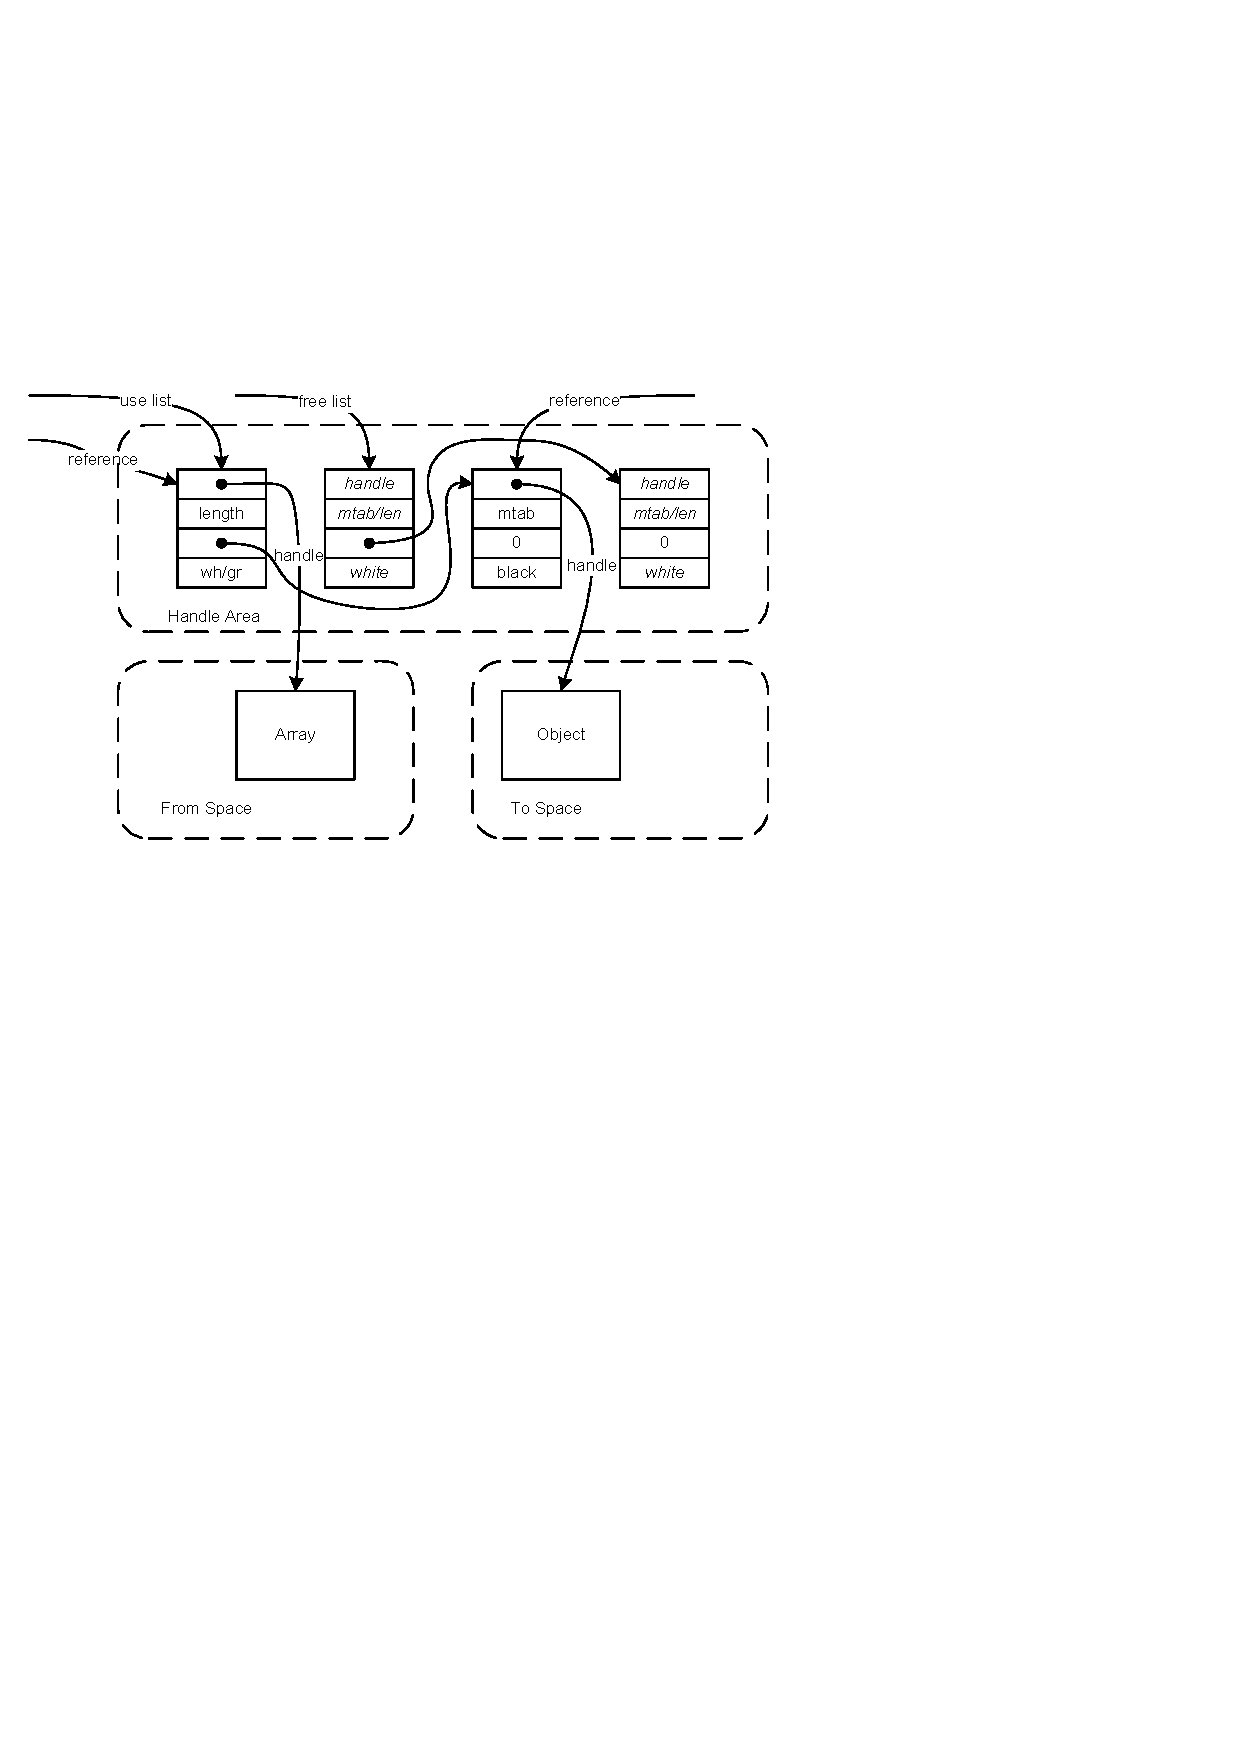
\includegraphics{jvm/handles}
  \caption{Heap layout with the handle area}\label{fig:handles}
\end{figure*}


\subsection{Implementation}

Our collector is an incremental collector with a
snapshot-at-the-beginning write barrier \cite{gc:yuasa90}. The GC is
based on the copy collector by Cheney \cite{gc:cheney70} and the
incremental version by Baker \cite{gc:baker78}. To avoid the
expensive read barrier in Baker's collector we perform all object
copies concurrently by the collector. Therefore we name it
\emph{concurrent-copy} collector. We have implemented the
concurrent-copy GC on the Java processor JOP \cite{jop:thesis,
jop:jnl:jsa2007}. The whole collector, the \code{new} operation, and
the write barriers are implemented in Java (with the help of two
native functions for direct memory access). Only the copy operation
is optimized by a faster microcode implementation. Although we show
the implementation on a Java processor the GC is not JOP specific
and can also be implemented on a conventional processor.

\subsubsection{Heap Layout}

Figure~\ref{fig:handles} shows a symbolic representation of the heap
layout with the handle area and two semi-spaces, \emph{fromspace} and
\emph{tospace}. Not shown in this figure is the memory region for
runtime constants, such as class information or string constants.
This memory region although logically part of the heap is neither
scanned, nor copied by the GC. This constant area contains it's own
handles and all references into this area are ignored by the GC.

To simplify object move by the collector all objects are accessed
with one indirection, called the handle. The handle also contains
auxiliary object data structures, such as a pointer to the method
table or the array length. Instead of Baker's read barrier we have
an additional mark stack which is a threaded list within the handle
structure. An additional field (as shown in
Figure~\ref{fig:handles}) in the handle structure is used for a free
list and a use list of handles.

The indirection through a handle, although a very light-weight read
barrier, is usually still considered as a high overhead. \linebreak
Metronome \cite{Bacon03} uses a forwarding pointer as part of the
object and performs forwarding \emph{eagerly}. Once the pointer is
forwarded subsequent uses of the reference can be performed on the
direct pointer till a GC preemption point. This optimization is
performed by the compiler.

We use a hardware based optimization\footnote{We have implemented it
for array access, but applying this optimization for field access is
straight forward.} for this indirection \cite{jop:oohw:jtres2007}.
The indirection is unconditionally performed in the memory access
unit. Furthermore, null pointer check (and array bounds check) is
done in parallel to this indirection.

There are two additional benefits from an explicit handle area instead of a
forwarding pointer: (a) access to the method table or array size needs no
indirection, and (b) the forwarding pointer and the auxiliary data
structures do not need to be copied by the GC.

The fixed handle area is not subject to fragmentation as all handles
have the same size and are recycled at a sweep phase with a simple
free list. However, the reserved space has to be sized (or the GC
period adapted) for the maximum number of objects that are live or
are floating garbage.


\subsubsection{The Collector}

The collector is scheduled periodically at the lowest priority and
within each period it performs following steps:
\begin{description}
    \item[Flip] An atomic flip exchanges the roles of tospace and
    fromspace.
    \item[Mark roots] All static references are pushed onto the mark
    stack. Only a single push operation needs to be atomic. As the
    thread stacks are empty we do not need an atomic scan of thread
    stacks.
    \item[Mark and copy] An object is popped from the mark stack,
    all referenced objects, which are still white, are pushed on the
    mark stack, the object is copied to tospace and the handle
    pointer is updated.
    \item[Sweep handles] All handles in the use list are checked if
    they still point into tospace (black objects) or can be added to
    the handle free list.
    \item[Clear fromspace] At the end of the collector work the
    fromspace that contains only white objects is initialized with
    zero. Objects allocated in that space (after the next flip) are
    already initialized and allocation can be performed in constant
    time.
\end{description}
%
The longest atomic operation is the copy of an object or array.  To
reduce blocking time, we plan to implement an array\footnote{Since
objects are typically small, this optimization is likely to pay off
only for arrays.} copy and access hardware module within JOP. The
hardware can perform copies in an interruptible fashion, and records
the copy position on an interrupt. On an array access the hardware
knows whether the access should go to the already copied part in the
tospace or in the not yet copied part in the fromspace. It has to be
noted that splitting larger arrays into smaller chunks, as done in
Metronome~\cite{Bacon03} and in the GC for the
JamaicaVM~~\cite{gc:siebert:phd}, is a software option to reduce the
blocking time.

The collector has two modes of operation: one for the initialization
phase and one for the mission phase. At the initialization phase it
operates in a stop-the-world fashion and gets invoked when a memory
request cannot be satisfied. In this mode the collector scans the
stack of the single thread conservatively. It has to be noted that
each reference points into the handle area and not to an arbitrary
position in the heap. This information is considered by the GC to
distinguish pointers from primitives. Therefore the chance to keep
an object artificial alive is low.

As part of the mission start one stop-the-world cycle is performed
to clean up the heap from garbage generated at initialization. From
that point on the GC runs in concurrent mode in it's own thread and
omits scanning of the thread stacks.

\subsubsection{The Mutator}

The coordination between the mutator and the collector is performed
within the \code{new} and \code{newarray} bytecodes and within write
barriers for JVM bytecodes \code{putfield} and \code{putstatic} for
reference fields, and bytecode \code{aastore}.

\paragraph{Allocation}

Objects are allocated black (in tospace). In non real-time
collectors it is more common to allocate objects white. It is argued
\cite{gc:dijkstra78} that objects die young and the chances are high
that the GC never needs to touch them. However, in the worst case no
object that is created and becomes garbage during the GC cycle can
be reclaimed. Those floating garbage will be reclaimed in the next
GC cycle. Therefore, we do not benefit from the white allocation
optimization in a real-time GC. Allocating a new object black has
the benefit that those objects do not need to be copied. The same
argument applies to the chosen write barrier. The following code
shows our simple implementation of bytecode \code{new}:

\begin{samepage}
{\small
\begin{verbatim}
synchronized (mutex) {
    // we allocate from the upper part
    allocPtr -= size;
    ref = getHandle(size);
    // mark as object
    Native.wrMem(IS_OBJ, ref+OFF_TYPE);
    // pointer to method table in the handle
    Native.wrMem(cons+CLASS_HEADR, ref+OFF_MTAB_ALEN);
}
\end{verbatim}
}
\end{samepage}

As the old fromspace is cleared by the GC we do not need to
initialize the new object and perform \code{new} in constant time.
The methods \code{Native.rdMem()} and \code{Native.wrMem()} provide
direct access to the main memory. Only those two native methods are
necessary for an implementation of a GC in pure Java.

\paragraph{Write Barriers}

A snapshot-at-begin write barrier synchronizes the mutator with the
collector on a reference store into a static field, an object field,
or an array. The \emph{to be overwritten} field is pushed on the
mark stack when it points to a white object. The following code
shows the implementation of \code{putfield} for reference fields:

{\small
\begin{verbatim}
private static void f_putfield_ref(int ref, int val,
                                    int index) {

    if (ref==0) {
        throw new NullPointerException();
    }
    synchronized (GC.mutex) {
        // handle indirection
        ref = Native.rdMem(ref);
        // snapshot-at-beginning barrier
        int oldVal = Native.rdMem(ref+index);
        if (oldVal!=0 &&
            Native.rdMem(oldVal+GC.OFF_SPACE)!=GC.toSpace) {

            GC.push(oldVal);
        }

        Native.wrMem(val, ref+index);
    }
}
\end{verbatim}
}

The shown code is part of a special class (\code{com.jopdesign.sys.JVM})
where Java bytecodes that are not directly implemented by JOP can be
implemented in Java \cite{jop:thesis}. All \code{putfield} bytecodes are
replaced by quick variants on class linking. During this step also
\code{putfield} instructions for references and double-word length fields
(\code{double} and \code{long}) are replaced by special
bytecodes. Therefore, the code shows the special bytecode
\code{putfield\_ref}.



\subsection{Evaluation}

To evaluate our proposed real-time GC we execute a simple test
application on JOP and measure the release time jitter of high
priority threads. The test setup consists of JOP implemented in an
Altera Cyclone FPGA clocked at 100~MHz. The main memory is a 1~MB
SRAM with an access time of two clock cycles. JOP is configured with
a 4~KB method cache (a special form of instruction cache) and a 128
entry stack cache. No additional data cache is used.

\subsubsection{Measuring Release Jitter}

Our main concern on garbage collection in real-time systems is the
blocking time introduced  by the GC due to atomic code sections.
This blocking time will be seen as release time jitter on the
real-time threads. Therefore we want to measure this jitter.

\begin{figure}
{\small
\begin{verbatim}
public boolean run() {

    int t = Native.rdMem(Const.IO_US_CNT);
    if (!notFirst) {
        expected = t+period;
        notFirst = true;
    } else {
        int diff = t-expected;
        if (diff>max) max = diff;
        if (diff<min) min = diff;
        expected += period;
    }
    work();

    return true;
}
\end{verbatim} }
    \caption{Measuring release time jitter}
    \label{lst:measure}
\end{figure}

Figure~\ref{lst:measure} shows how we measure the jitter. Method
\code{run()} is the main method of the real-time thread and executed
on each periodic release. Within the real-time thread we have no
notion about the start time of the thread. As a solution we measure
the actual time on the first iteration and use this time as first
release time. Each iteration the expected time, stored in the
variable \code{expected}, is incremented by the \code{period}. In
each iteration (except the first one) the actual time is compared
with the expected time and the maximum value of the difference is
recorded.

As noted before, we have no notion about the \emph{correct} release
times. We measure only relative to the first release. When the first
release is delayed (due to some startup code or interference with a
higher priority thread) we have a positive offset in
\code{expected}. On an exact release in a later iteration the time
difference will be negative (in \code{diff}). Therefore, we also
record the minimum value for the difference between the actual time
and the expected time. The maximum measured release jitter is the
difference between \code{max} and \code{min}.

To provide a baseline we measure the release time jitter of a single
real-time thread (plus an endless loop in the \code{main} method as
an idle non-real-time background thread). No GC thread is scheduled.
The code is similar to the code in in Figure~\ref{lst:measure}. A
stop condition is inserted that prints out the minimum and maximum
time differences measured after 1 million iterations.

\begin{table}
    \centering
    \begin{tabular}{rr}
    \toprule
    Period & Jitter \\
    \midrule
    200 $\mu$s & 0 $\mu$s \\
    100 $\mu$s & 0 $\mu$s \\
    50 $\mu$s & 17 $\mu$s \\
    \bottomrule
    \end{tabular}
    \caption{Release jitter for a single thread}
    \label{tab:single}
\end{table}

Table~\ref{tab:single} shows the measured jitter for different
thread periods. We observed no jitter for periods of 100~$\mu$s and
longer. At a period of 50~$\mu$s the scheduler introduces a
considerable amount of jitter. From this measurement we conclude
that 100~$\mu$s is the practical shortest period we can handle with
our system. We will use this period for the high-priority real-time
thread in the following measurement with an enabled GC.

\subsubsection{Measurements}

The test application consisting of three real-time threads
($\tau_{hf}$, $\tau_{p}$, and $\tau_{c}$), one logging thread
$\tau_{log}$, and the GC thread $\tau_{gc}$. All three real-time
threads measure the difference between the expected release time and
the actual release time (as shown in Figure~\ref{lst:measure}). The
minimum and maximum values are recorded and regularly printed to the
console by the logging thread $\tau_{log}$. Table~\ref{tab:exp}
shows the release parameters for the five threads. Priority is
assigned deadline monotonic. Note that the GC thread has a shorter
period than the logger thread, but a longer deadline. For our
approach to work correctly the GC thread \emph{must} have the lowest
priority. Therefore all other threads with a longer period than the
GC thread must be assigned a shorter deadline.

\begin{table}
    \centering
    \begin{tabular}{lrrr}
    \toprule
    Thread & Period & Deadline & Priority \\
    \midrule
    $\tau_{hf}$ & 100 $\mu$s & 100 $\mu$s & 5 \\
    $\tau_{p}$ &  1 ms & 1 ms & 4 \\
    $\tau_{c}$ & 10 ms & 10 ms & 3 \\
    $\tau_{log}$ & 1000 ms & 100 ms & 2 \\
    $\tau_{gc}$ & 200 ms & 200 ms & 1 \\
    \bottomrule
    \end{tabular}
    \caption{Thread properties of the test program}
    \label{tab:exp}
\end{table}

Thread $\tau_{hf}$ represents a high-frequency thread without
dynamic memory allocation. This thread should observe minimal
disturbance by the GC thread.

The threads $\tau_{p}$ and $\tau_{c}$ represent a producer/consumer
pair that uses dynamically allocated memory for communication. The
producer appends the data at a frequency of 1~kHz to a simple list.
The consumer thread runs at 100~Hz and processes all currently
available data in the list and removes them from the list. The
consumer will process between 9 and 11 elements (depending on the
execution time of the consumer and the thread phasing).

It has to be noted that this simple and common communication pattern
cannot be implemented with the scoped memory model of the RTSJ.
First, to use a scope for communication, we have to keep the scope
alive with a \emph{wedge} thread \cite{conf/isorc/PizloFHV04} when
data is added by the producer. We would need to notify this wedge
thread by the consumer when all data is consumed. However, there is
no single instant available where we can \emph{guarantee} that the
list is empty. A possible solution for this problem is described in
\cite{conf/isorc/PizloFHV04} as \emph{handoff} pattern. The pattern
is similar to double buffering, but with an explicit copy of the
data. The elegance of a simple list as buffer queue between the
producer and the consumer is lost.

Thread $\tau_{log}$ is not part of the real-time systems simulated
application code. Its purpose is to print the minimum and maximum
differences between the measured and expected release times (see
former section) of threads $\tau_{hf}$ and $\tau_{p}$ to the console
periodically.

Thread $\tau_{gc}$ is a standard periodic real-time thread executing
the GC logic. The GC thread period was chosen quite short in that
example. A period in the range of seconds would be enough for the
memory allocation by $\tau_{p}$. However, to stress the interference
between the GC thread and the application threads we artificially
shortened the period.

\begin{table}
    \centering
    \begin{tabular}{lr}
    \toprule
    Threads & Jitter \\
    \midrule
    $\tau_{hf}$ & 0 $\mu$s \\
    $\tau_{hf}$, $\tau_{log}$ & 7 $\mu$s \\
    $\tau_{hf}$, $\tau_{log}$,$\tau_{p}$,$\tau_{c}$ & 14 $\mu$s \\
    $\tau_{hf}$, $\tau_{log}$,$\tau_{p}$,$\tau_{c}$,$\tau_{gc}$ & 54 $\mu$s \\
    \bottomrule
    \end{tabular}
    \caption{Jitter measured on a 100~MHz processor for the high priority thread in different configurations}
    \label{tab:jitter}
\end{table}
As a first experiment we run only $\tau_{hf}$ and the logging thread
$\tau_{log}$ to measure jitter introduced by the scheduler. The
maximum jitter observed for $\tau_{hf}$ is 7 $\mu$s -- the blocking
time of the scheduler.

In the second experiment we run all threads except the GC thread.
For the first 4 seconds we measure a maximum jitter of 14~$\mu$s for
thread $\tau_{hf}$. After those 4 seconds the heap is full and GC is
necessary. In that case the GC behaves in a stop-the-world fashion.
When a new object request cannot be fulfilled the GC logic is
executed in the context of the allocating thread. As the bytecode
\code{new} is itself in an atomic region the application is blocked
until the GC finishes. Furthermore, the GC performs a conservative
scan of all thread stacks. We measure a release delay of 63~ms for
all threads due to the blocking during the full collection cycle.
From that measurement we can conclude for the sample application and
the available main memory: (a) the measured maximum period of the GC
thread is in the range of 4 seconds; (b) the estimated execution
time for one GC cycle is 63~ms. It has to be noted that measurement
is not a substitution for static timing analysis. Providing WCET
estimates for a GC cycle is a challenge for future work.

In our final experiment we enabled all threads. The GC is scheduled
periodically at 200~ms as the lowest priority thread -- the scenario
we argue for. The GC logic is set into the concurrent mode on
mission start. In this mode the thread stacks are not scanned for
roots. Furthermore when an allocation request cannot be fulfilled
the application is stopped. This radical stop is intended for
testing. In a more tolerant implementation either a out-of-memory
exception can be thrown or the requesting thread has to be blocked,
it's thread stack scanned and released when the GC has finished it's
cycle.

We ran the experiment for several hours and recorded the maximum
release jitter of the real-time threads. For this test we used
slightly different periods (prime numbers) to avoid the regular
phasing of the threads. The harmonic relation of the original
periods can lead to too optimistic measurements. The applications
never ran out of memory. The maximum jitter observed for the high
priority task $\tau_{hf}$ was 54~$\mu$s. The maximum jitter for task
$\tau_{p}$ was 108~$\mu$s. This higher value on $\tau_{p}$ is
expected as the execution interferes with the execution of the
higher priority task $\tau_{hf}$.

\subsubsection{Discussion}


With our measurements we have shown that quite short blocking times
are achievable. Scheduling introduces a blocking time of about
7--14~$\mu$s and the GC adds another 40~$\mu$s resulting in a
maximum jitter of the highest priority thread of 54~$\mu$s. In our
first implementation we performed the object copy in pure Java,
resulting in blocking times around 200~$\mu$s. To speedup the copy
we moved this function to microcode. However, the microcoded
\emph{memcpy} still needs 18 cycles per 32-bit word copy. Direct
support in hardware can lead to a copy time of 4--5 clock cycles per
word.

The maximum blocking time of 54~$\mu$s on a 100 MHz processor is less than
blocking times reported for other solutions.

%% --- THIS IS GOING TO GET US INTO TROUBLE
%% Blocking time for Metronome
%% (called pause times in the papers) is reported to be 6~ms
%% \cite{gc:jtres:metronome} on a 500~MHz PowerPC at 50\% CPU
%% utilization. Those large blocking times are due to the scheduling of the GC
%% at the highest priority with a polling based yield within the GC thread. A
%% fairer comparison is against the \emph{jitter} of the pause time. In
%% \cite{gc:bacon05} the variation of the pause time is given between
%% 500~$\mu$s and 2.4~ms on a 1~Ghz machine. It should be noted that Metronome
%% is a GC intended for mixed real-time systems whereas we aim only for hard
%% real-time systems.

%% Robertz performed a similar measurement as we did for his thesis
%% \cite{gc:robertz:thesis} with a time-triggered GC on a 350~MHz
%% PowerPC. He measured a maximum jitter of 20~$\mu$s ($\pm10$~$\mu$s)
%% for a high priority task with a period of 500~$\mu$s.

%% It has to be noted that our experiment is a small one and we need
%% more advanced real-time applications for the evaluation of real-time
%% GC. The problem is that it is hard to find even static based
%% real-time application benchmarks (at least applications written for
%% safety critical Java). Running standard benchmarks that measure
%% average case performance (e.g., SPEC jvm98) is not an option to
%% evaluate a real-time collector.

%SUN RTS jitter +- 10us, but heap schedulables 100us

%lund release time jitter 40us - from where do I have this number

%\url{http://www.robot.lth.se/java/} compiler

%read \url{http://www.ulb.ac.be/di/ssd/goossens/RTS05.pdf}

%\subsection{Future Enhancements}

Although we measured a low blocking time in our experiment we think
there is room for improvements. As a first enhancement we will
implement a hardware \emph{memcpy} in the memory unit of JOP to
reduce the blocking time. However, for very large arrays the
resulting blocking time may still be too large. A common solution is
to break up arrays into smaller chunks sometimes called Arraylets
\cite{Bacon03}. However, this comes at a more complex array access
with a higher cost.

As we are running our GC on a soft-core Java processor our design
space is larger and we can consider implementing a function unit
that supports incremental copy. This copy unit will be integrated
with the array (field) access unit. On a timer interrupt (for a
scheduling decision) the memory copy will also be interrupted and
the application thread can run. The copy/access unit remembers the
copy position and will redirect the array/field access either to
fromspace or to tospace.

Another option is a full hardware implementation of the GC. The
proposed algorithm is not very complex and should result in a not
too complex hardware. However, this design direction should be
carefully evaluated against a way simpler parallel solution: running
the GC on one CPU of a chip multiprocessor version of JOP.

\subsection{Summary} \label{sec:concl}

In this paper we have presented a real-time garbage collector for
safety critical Java. Our collector is scheduled as a normal
real-time thread and, according to it's deadline, assigned the
lowest priority in the system. The restrictions from the SCJ
programming model and the low priority result in two advantages: (a)
avoidance of stack root scanning and (b) short blocking time of high
priority threads. We have implemented the proposed GC on the Java
processor JOP. At 100~MHz we measured 40~$\mu$s maximum blocking
time introduced by the GC thread.

As future work we plan to implement the presented GC in
Ovm~\cite{tecs:06} for a safety critical Heaplet. A critical
operation for a concurrent, compacting GC is the atomic copy of
large arrays. We consider to extend JOP with a copy unit that can be
interrupted. This unit is integrated with the array access unit and
will redirect the access to either fromspace or tospace depending on
the array index and the value of the copy pointer.




%%% I don't really expect the reviewers to download the software.

%MS: I know, but they could ;-) That's a tick I have. I've seen too
%many papers that are written without an implementation to backup the
%ideas (even PhD thesis).
%
%I would like to see more pressure on this issue e.g., give some
%extra points in the review when the SW is available for download. In
%our field it should be easy to reevaluate the results and to redo
%the measurements that are presented in the paper (way easier than in
%other fields e.g., Physics). I think this would enhance the quality
%of many papers ;-)


\subsection*{Note to the Reviewer}

The version of JOP and the RT garbage collector are available from
the CVS: {\small
\begin{verbatim}
cvs -d :pserver:anonymous@cvs.opencores.org:/cvsroot/anonymous \
    -z9 co -P -r jtres2007_submission jop
\end{verbatim}
} A simple \code{make} builds the whole processor and runs a
\emph{Hello World} program. The GC example from this paper is built
and downloaded with: {\small
\begin{verbatim}
    make japp -e P1=test P2=gcinc P3=Latency
\end{verbatim}
}

Note that the default configuration of JOP in the CVS is for 80~MHz
for easier compilation of the CPU in Quartus. Therefore, the
reported latencies will be 20\% higher. We tweaked the compilation
process to achieve a clock frequency of 100~MHz as used in the
example.

%\pagebreak
%\pagebreak
\section{Some notes}

\emph{MS: not the actual text, but to make ideas clearer for me.}

For a concurrent (incremental) GC some coordination between the
collector and the mutator are necessary. The usual solution is a
write barrier in the mutator to not foil the collector.

\begin{description}
    \item[Snapshot-at-beginning] Keep the object graph as it was at
    the the GC start
    \begin{itemize}
        \item Save to-be-overwritten pointer
        \item More conservative -- not an issue for RT as worst case
        counts
        \item Allocate black
        \item New objects (e.g.\ new stack frames) do not need a
        write barrier
        \item Optimization: with atomic root scan of the thread
        stacks no write barrier is necessary for locals and the JVM
        stack
    \end{itemize}
    \item[Incremental update] \emph{Help} the GC by doing some collection
    work in the mutator
    \begin{itemize}
        \item Preserve strong tri-color invariant (no pointer from
        black to white objects)
        \item On black to white shade the white object (shade the
        black is unusual)
        \item Allocate black (in contrast to \cite{gc:dijkstra78})
        \item Needs write barriers for locals -- is that true?
        \item Less conservative than snapshot-at-beginning
    \end{itemize}
\end{description}

The usual choice is snapshot-at-beginning with atomic root scan of
all thread stacks to avoid write barriers on locals -- \emph{Is this
true?}

\subsection{Write Barriers}

Assume following assignment:

\begin{verbatim}
    o.r = ref;
\end{verbatim}

There are three references involved that can be manipulated:
\begin{itemize}
    \item The old value of o.r
    \item The new value ref
    \item The object o
\end{itemize}

The three possible write barriers are:

Snapshot-at-beginning/weak tri-color invariant:
\begin{verbatim}
    if (white(o.r)) markGrey(o.r);
    o.r = ref;
\end{verbatim}

Incremental/strong tri-color invariant with push forward
\begin{verbatim}
    if (black(o) && white(ref)) markGrey(ref);
    o.r = ref;
\end{verbatim}
Optimization: Check only white(ref).

Incremental/strong tri-color invariant with push back
\begin{verbatim}
    if (black(o) && white(ref)) markGrey(o);
    o.r = ref;
\end{verbatim}

We have no stack roots when the collector runs. Therefore we can use
the incremental write barrier for object fields only. \emph{Is that
write barrier simpler than the snapshot-at-beginning?}



\subsection{Further Notes}

We go for a RTGC that is scheduled periodically with the lowest
priority. Therefore the GC will never preempt a real-time thread.
This results is following features of the system:

\begin{itemize}
    \item No stack scanning is necessary, which is usually atomic
    \item No write barriers for local variables needed
    \item No GC preemption points, which are used to avoid too many
    write barriers
\end{itemize}

Some more points for this paper:

\begin{itemize}
    \item Sketch the scheduling analysis from the ISORC 2006 paper
    \cite{jop:rtgc_sched}
\end{itemize}

Talk about:\begin{itemize}
    \item GC zaps semi-space for fast allocation
    \item Measure allocation time
    \item Measure zap time
\end{itemize}

\subsection{Describe}


\begin{itemize}
    \item Lowest priority (= background task)
    \item Copying collector
    \item Indirection with handles
    \item Use a mark stack within the handles
    \item Synchronization
    \item Mutator barriers
    \item Atomic copy (issue for large arrays -- HW can help)
    \item putfield/putstatic optimization for references through
    bytecode rewriting
    \item GC is stop-the-world at initialization phase
    \item Special collection cycle on mission start to move static
    data to a non collected, but scanned, area. Similar to RTSJ
    immortal, but pointers into the heap are allowed -- we should
    name it \emph{static} memory.
    \item Synchronization with a simple turn off interrupt
    \item talk about WCMC analysis -- allocation is easy, release is
    the hard part
    \item collector written in Java
\end{itemize}


\subsection{Code Snippets}

\emph{MS: Shall we provide some pseudo code for the GC, new and the
write barriers?}

Code from the GC implementation for JOP. When used we should
translate it to a more readable pseudo code.

Flip:
\begin{verbatim}
    synchronized (mutex) {
        useA = !useA;
        if (useA) {
            copyPtr = heapStartA;
            fromSpace = heapStartB;
            toSpace = heapStartA;
        } else {
            copyPtr = heapStartB;
            fromSpace = heapStartA;
            toSpace = heapStartB;
        }
        allocPtr = copyPtr+semi_size;
    }
\end{verbatim}


Root marking:
\begin{verbatim}
    int addr = Native.rdMem(addrStaticRefs);
    int cnt = Native.rdMem(addrStaticRefs+1);
    for (i=0; i<cnt; ++i) {
        push(Native.rdMem(addr+i));
    }
\end{verbatim}

Push:
\begin{verbatim}
    if (Native.rdMem(ref+OFF_GREY)!=0) {
        return;
    }
    if (Native.rdMem(ref+OFF_GREY)==0) {
        // pointer to former gray list head
        Native.wrMem(greyList, ref+OFF_GREY);
        greyList = ref;
    }
\end{verbatim}

Mark and Copy:
\begin{verbatim}
    for (;;) {

        // pop one object from the gray list
        synchronized (mutex) {
            ref = greyList;
            if (ref==GREY_END) {
                break;
            }
            greyList = Native.rdMem(ref+OFF_GREY);
            Native.wrMem(0, ref+OFF_GREY);      // mark as not in list
        }



        // push all childs

        // get pointer to object
        int addr = Native.rdMem(ref);
        int flags = Native.rdMem(ref+OFF_TYPE);
        if (flags==IS_REFARR) {
            // is an array of references
            int size = Native.rdMem(ref+OFF_MTAB_ALEN);
            for (i=0; i<size; ++i) {
                push(Native.rdMem(addr+i));
            }
        } else if (flags==IS_OBJ){
            // it's a plain object
            // get pointer to method table
            flags = Native.rdMem(ref+OFF_MTAB_ALEN);
            // get real flags
            flags = Native.rdMem(flags+MTAB2GC_INFO);
            for (i=0; flags!=0; ++i) {
                if ((flags&1)!=0) {
                    push(Native.rdMem(addr+i));
                }
                flags >>>= 1;
            }
        }

        // now copy it - color it BLACK


        int size = Native.rdMem(ref+OFF_SIZE);
        synchronized (mutex) {
            // update object pointer to the new location
            Native.wrMem(copyPtr, ref+OFF_PTR);
            // set it BLACK
            Native.wrMem(toSpace, ref+OFF_SPACE);
            // copy it
            for (i=0; i<size; ++i) {
                Native.wrMem(Native.rdMem(addr+i), copyPtr+i);
            }
            copyPtr += size;
        }
    }
\end{verbatim}

Sweep handles:
\begin{verbatim}
    synchronized (mutex) {
        ref = useList;      // get start of the list
        useList = 0;        // new uselist starts empty
    }

    while (ref!=0) {

        int next = Native.rdMem(ref+OFF_NEXT);
        // a BLACK one
        if (Native.rdMem(ref+OFF_SPACE)==toSpace) {
            // add to used list
            synchronized (mutex) {
                Native.wrMem(useList, ref+OFF_NEXT);
                useList = ref;
            }
        // a WHITE one
        } else {
            // add to free list
            synchronized (mutex) {
                Native.wrMem(freeList, ref+OFF_NEXT);
                freeList = ref;
                Native.wrMem(0, ref+OFF_PTR);
            }
        }
        ref = next;
    }
\end{verbatim}

Zap fromspace:
\begin{verbatim}
        for (int i=fromSpace; i<fromSpace+semi_size; ++i) {
            Native.wrMem(0, i);
        }
\end{verbatim}
